
\documentclass[submission,copyright,creativecommons]{eptcs}
\providecommand{\event}{ACT 2026}
\usepackage{breakurl}
\usepackage{underscore}

\usepackage{amsmath,amssymb,amsthm}
\usepackage{tikz-cd}
\usepackage{tikz}
\usetikzlibrary{decorations.pathreplacing,positioning}
\usepackage{listings}
\usepackage{xcolor}
\usepackage{booktabs}

% eptcs+mathptmx can request OT1/ptm/m/scit; map it to small caps to avoid font warnings.
\DeclareFontShape{OT1}{ptm}{m}{scit}{<->ssub * ptm/m/sc}{}

\newtheorem{definition}{Definition}
\newtheorem{theorem}{Theorem}
\newtheorem{proposition}{Proposition}
\newtheorem{lemma}{Lemma}

\lstset{
  basicstyle=\ttfamily\small,
  keywordstyle=\color{blue},
  commentstyle=\color{gray},
  breaklines=true,
  frame=single,
  columns=flexible
}

\title{Functorial Composition over Task Decomposition: \\ A Categorical Kernel for AI-Human Computation}
\author{Anonymous Author
\institute{mo:os Project}
\email{author@example.com}
}
\def\titlerunning{Functorial Composition over Task Decomposition}
\def\authorrunning{A. Author}

\begin{document}
\maketitle

\begin{abstract}
Multi-agent AI frameworks decompose tasks top-down, producing orchestrations
that lack formal structural guarantees. We present \texttt{mo:os}, a runtime
kernel realized as a symmetric monoidal category where computational entities
are objects and state transitions are exactly four natural transformations
(\textsc{Add}, \textsc{Link}, \textsc{Mutate}, \textsc{Unlink}) over a typed
graph. Applying Lawvere's functorial semantics, \texttt{mo:os} separates
syntax (a JSON-schema-validated ontology of 21 object kinds and 16 morphism
types) from semantics (a deterministic Go execution engine implementing a
catamorphism $\mathit{state}(t) = \mathit{fold}(\mathit{log}[0..t])$). By
restricting LLMs to emit typed morphisms rather than orchestration plans,
complex behavior emerges from bottom-up operadic composition rather than
unstructured decomposition. We formalize the Container Category, prove closure
under parallel and sequential wiring, present the Recursive Semantic Bridge as
a structure-preserving functor, construct a natural transformation from the
kernel to the Model Context Protocol, and report implementation metrics from a
working kernel: approximately 4{,}000 lines of Go, 118 nodes, 131 wires, 17 HTTP
endpoints, an MCP bridge with 5 tool schemas, and deterministic replay from an
append-only morphism log.
\end{abstract}

%% -----------------------------------------------------------------
\section{Introduction}
\label{sec:intro}

The rapid adoption of large language models (LLMs) as orchestrators of
multi-agent systems has exposed a fundamental architectural tension: the
frameworks that decompose tasks---LangChain, CrewAI, AutoGen, and their
successors---rely on the LLM's embedding space to simultaneously serve as
computation engine, state router, and correctness oracle. This conflation
produces what we term the \emph{semantic bottleneck}: as task complexity grows,
recombination of sub-results depends on ad-hoc aggregation that is brittle to
hallucination and context-window overflow.

We propose an inversion of control. Rather than asking the LLM to
\emph{orchestrate}, we restrict it to the role of a \emph{Fuzzy Processing
Unit} (FPU) that emits candidate morphisms over a strictly typed categorical
state machine. The deterministic kernel accepts or rejects these morphisms
against a semantic registry before committing them to an append-only log. This
separation---syntax from semantics, in the sense of Lawvere
\cite{lawvere1963}---yields structural guarantees that top-down decomposition
cannot provide.

\texttt{mo:os} is an open-source (MIT) runtime kernel, implemented in Go,
that realizes this architecture. Its categorical foundation draws on Fong and
Spivak's compositional framework \cite{fong2018}, Spivak's operadic wiring
diagrams \cite{spivak2013,spivak2013operad}, and Yau's finite presentation
results for wiring diagram operads \cite{yau2018}. Unlike Catlab (scientific
computing) or Statebox (blockchain consensus) \cite{statebox2019}, \texttt{mo:os}
targets the operational gap between LLM inference and industrial graph
state management.

\paragraph{Contributions.}
\begin{enumerate}
  \item We define the \emph{Container Category} $\mathcal{C}$ and prove it is
        closed under parallel and sequential wiring (Section~\ref{sec:container}).
  \item We prove the \emph{Authority Filtration} theorem and establish a
        Galois connection between the causal birth order and the stratum
        classification, showing that governance is a structural property of
        the morphism log (Section~\ref{sec:container}).
  \item We formalize four invariant natural transformations and the operadic
        validation algebra that constrains them (Section~\ref{sec:bottleneck}).
  \item We construct the \emph{Recursive Semantic Bridge} as a
        structure-preserving functor $F\colon \mathbf{Syn} \to \mathbf{Sem}$
        and show that hydration stages correspond to strata of realization
        (Section~\ref{sec:bridge}).
  \item We formalize the LLM as an endofunctor rather than an orchestrator,
        and define a benchmark functor mapping providers to a metric space
        (Section~\ref{sec:bridge}).
  \item We present \emph{System~3} DAG reasoning as an extension of
        LogicGraph \cite{logicgraph2025} (Section~\ref{sec:system3}).
  \item We construct the MCP bridge as a natural transformation from kernel
        categories to tool-schema categories and define pipeline complexity
        metrics with formal cost bounds (Section~\ref{sec:implementation}).
  \item We report metrics from a working implementation: approximately 4{,}000
        lines of Go, 118 nodes and 131 wires post-hydration, deterministic
        catamorphic replay, an MCP bridge with 5 tools, and a 21-kind ontology
        validated by an operad registry (Section~\ref{sec:implementation}).
\end{enumerate}

%% -----------------------------------------------------------------
\section{Background: Functorial Semantics and Operadic Composition}
\label{sec:background}

\subsection{Lawvere's Functorial Semantics}

Lawvere \cite{lawvere1963} established that an algebraic theory $\mathbf{T}$
can be separated from its models by defining models as product-preserving
functors $M\colon \mathbf{T} \to \mathbf{Set}$. This separation of syntax
(the theory) from semantics (the model) is the conceptual foundation of
\texttt{mo:os}: the JSON ontology is our syntax category, and the Go kernel is
a model that evaluates it.

\subsection{Operadic Wiring Diagrams}

Spivak \cite{spivak2013} formalized wiring diagrams as an operad
$\mathcal{W}$ where operations describe how boxes with typed ports are
interconnected. Rupel and Spivak \cite{spivak2013operad} extended this to
temporal wiring diagrams with directed, length-bearing wires suitable for
modeling dynamic information flow. Yau \cite{yau2018} proved that
$\mathcal{W}$ admits a finite presentation with 8 generators and 28 relations.

In \texttt{mo:os}, the 16 morphism types of our ontology correspond to
generators of a sub-operad of $\mathcal{W}$, and the semantic registry
enforces the operadic relations: each wire must connect admissible port types
with correct directionality.

\subsection{Dynamic Operads and Agent Composition}

Shapiro et al.\ \cite{shapiro2022} introduced \emph{dynamic operads} via the
monoidal double category $\mathbf{Org}$, showing how organized systems adapt
their operadic structure in response to internal and external pressures. This
framework supports the view of \texttt{mo:os} as a dynamic categorical system
where the graph topology evolves through morphism application while preserving
algebraic invariants.

Bonchi, Pavlovic, and Sobocinski \cite{bonchi2017functorial} extended
functorial semantics from algebraic to relational theories, providing tools for
reasoning about agent interactions as structure-preserving maps between
relational networks---a pattern we exploit in the \texttt{mo:os} wiring
algebra.

%% -----------------------------------------------------------------
\section{The Container Category}
\label{sec:container}

\begin{definition}[Container Category]
The \emph{Container Category} $\mathcal{C}$ has:
\begin{itemize}
  \item \textbf{Objects}: typed nodes $n = (\mathit{urn}, \tau, \sigma, \pi)$
        where $\mathit{urn}$ is a unique identifier, $\tau \in \mathcal{T}$ is
        a type drawn from the ontology ($|\mathcal{T}| = 21$), $\sigma \in
        \{S_0, \ldots, S_4\}$ is a stratum, and $\pi$ is a payload.
  \item \textbf{Morphisms}: directed wires $w\colon n_1 \to n_2$ specified by
        the 4-tuple $(\mathit{src}, p_s, \mathit{tgt}, p_t)$ where $p_s, p_t$
        are typed ports.
  \item \textbf{Identity}: for each node $n$, the identity wire
        $\mathrm{id}_n$ is the trivial self-loop (elided in practice).
  \item \textbf{Composition}: wires compose when the target port of one matches
        the source port of the next, subject to the operadic constraints of
        the semantic registry.
\end{itemize}
\end{definition}

The graph state at time $t$ is the carrier of the catamorphism:
\begin{equation}
\label{eq:cata}
\mathit{state}(t) = \mathrm{fold}\bigl(\mathit{log}[0..t],\; \varnothing,\;
\mathit{eval}\bigr)
\end{equation}
where $\varnothing$ is the empty graph (initial object) and $\mathit{eval}$
applies a single morphism envelope to produce a new state.

\begin{definition}[Stratum Lattice]
The five strata form a partial order:
\[
S_0\ (\text{Authored}) \leq S_1\ (\text{Validated}) \leq S_2\
(\text{Materialized}) \leq S_3\ (\text{Evaluated}) \leq S_4\ (\text{Projected})
\]
Higher strata may depend on lower strata; lower strata must not depend on
higher strata for meaning. $S_4$ projections are never ground truth.
\end{definition}

\begin{proposition}[Closure under Wiring]
\label{prop:closure}
Let $G_1, G_2$ be valid graph states in $\mathcal{C}$. The parallel
composition $G_1 \otimes G_2$ (disjoint union of nodes and wires) and the
sequential composition $G_1 \circ G_2$ (wire matching on shared ports) both
yield valid graph states in $\mathcal{C}$, provided all wires satisfy the
operadic constraints of the semantic registry.
\end{proposition}

\begin{proof}[Proof sketch]
Parallel composition preserves validity because disjoint union introduces no
new port conflicts. Sequential composition requires that matched ports have
compatible types and directions, which is enforced by the registry's
\texttt{ValidateLink} function checking source port direction (``out''), target
port direction (``in''), and target type membership in the source port's
admissible target set.
\end{proof}

\subsection{Ownership as Full Subcategory}

The OWNS morphism ($\mathit{MOR01}$) induces a forest structure on
$\mathcal{C}$. For any actor $a$, the \emph{scope} of $a$ is the full
subcategory $\mathcal{C}_a \hookrightarrow \mathcal{C}$ consisting of all
nodes transitively reachable from $a$ via OWNS wires. This is computed by
breadth-first search under a read lock, yielding all internal wires---those
whose source and target both lie in $\mathcal{C}_a$.

\subsection{Authority Filtration}
\label{subsec:authority}

The morphism log and the stratum lattice each induce a filtration of
$\mathcal{C}$, but these two filtrations are \emph{independent} and run in
opposite directions on the lower strata. Making this precise is the key
structural result of the paper.

\begin{definition}[Causal Filtration]
\label{def:causal-filtration}
Let the morphism log have $t$ entries. For each $k \in \{0, \ldots, t\}$,
let $\mathcal{C}_{\leq k}$ be the full subcategory of $\mathcal{C}$ whose
objects have been created by \textsc{Add} envelopes at log positions
$\leq k$. The chain
\[
\varnothing = \mathcal{C}_{\leq -1}
\hookrightarrow \mathcal{C}_{\leq 0}
\hookrightarrow \mathcal{C}_{\leq 1}
\hookrightarrow \cdots
\hookrightarrow \mathcal{C}_{\leq t} = \mathcal{C}
\]
is the \emph{causal filtration} of $\mathcal{C}$. Each step adds at most one
object (the node created by the \textsc{Add} at position $k$, if any).
\end{definition}

\begin{definition}[Stratum Filtration]
\label{def:stratum-filtration}
For each stratum $S_i$, let $\mathcal{C}^{\sigma}_{\leq i}$ be the full
subcategory of $\mathcal{C}$ whose objects have stratum $\leq S_i$. The chain
\[
\mathcal{C}^{\sigma}_{\leq 0} \hookrightarrow
\mathcal{C}^{\sigma}_{\leq 1} \hookrightarrow
\mathcal{C}^{\sigma}_{\leq 2} \hookrightarrow
\mathcal{C}^{\sigma}_{\leq 3} \hookrightarrow
\mathcal{C}^{\sigma}_{\leq 4} = \mathcal{C}
\]
is the \emph{stratum filtration} of $\mathcal{C}$ by full subcategories.
\end{definition}

The kernel self-seeds at boot: the first morphism in every log is
$\textsc{Add}(\mathit{urn\!:\!moos\!:\!kernel\!:\!wave\text{-}0})$, a node at
stratum $S_2$. Every subsequent node enters $\mathcal{C}$ via a finite
sequence of \textsc{Add} and \textsc{Link} morphisms traceable back to this
seed through the \emph{causal} filtration---not the stratum filtration.

\begin{theorem}[Authority Filtration]
\label{thm:authority}
Every node $n \in \mathrm{Ob}(\mathcal{C})$ has a finite causal path in the
morphism log to the kernel seed. Formally: for each $n$ with
$\mathrm{birth}(n) = k > 0$, there exists a \textsc{Link} morphism
$\ell\colon m \to n$ in the log with $\mathrm{birth}(m) < k$---that is, the
authorizing node $m$ already exists in $\mathcal{C}_{\leq k-1}$.
By induction, every node is connected to the seed by a finite chain of such
\textsc{Link} morphisms.
\end{theorem}

\begin{proof}[Proof sketch]
By construction of the boot sequence and the hydration pipeline. The kernel
seed at $S_2$ is the first \textsc{Add} (log position~0). Source nodes at
$S_1$ are seeded next via \textsc{Add} + \textsc{Link}(kernel, source).
Industry entities at $S_0$ enter later via \textsc{Add} +
\textsc{Link}(source, industry). Instance nodes at $S_2$ are hydrated via
\textsc{Add} + \textsc{Link}(industry, instance) or
\textsc{Link}(kernel, instance). Projections at $S_4$ are functor outputs.
At each step, the \textsc{Link} envelope's precondition (both endpoints must
exist) guarantees that the authorizing node has a strictly earlier birth
position. Since the log is finite, the inductive chain terminates at the seed.
\end{proof}

Crucially, the authorizing \textsc{Link} need not respect the stratum order:
the seed at $S_2$ authorizes source nodes at $S_1$ and industry entities at
$S_0$. Authority flows \emph{down} the stratum lattice while semantic
dependency flows \emph{up}. This contravariance is not a defect but a
structural feature, which we now make precise.

\begin{proposition}[Contravariant Orders]
\label{prop:contravariant}
Let $\mathrm{complete}\colon \Sigma \to \mathbb{N}$ map each stratum $S_i$ to
the last log position at which a node of stratum $S_i$ is created, and let
$\mathrm{filled}\colon \mathbb{N} \to \Sigma$ map each log position $k$ to
the highest stratum $S_i$ such that all $S_i$-nodes have
$\mathrm{birth} \leq k$. Then $\mathrm{filled} \dashv \mathrm{complete}$
is a Galois connection between $(\mathbb{N}, \leq)$ and
$(\Sigma, \leq)^{\mathrm{op}}$:
\[
\mathrm{filled}(k) \geq S_i
\quad\Longleftrightarrow\quad
k \geq \mathrm{complete}(S_i).
\]
In particular, the stratum order and the causal birth order are contravariant
on the lower strata: the kernel seed is causally initial
($\mathrm{birth} = 0$) but resides at $S_2$, while $S_0$ industry entities
are causally posterior but immutable.
\end{proposition}

\begin{proof}[Proof sketch]
Both maps are well-defined on a finite log. The equivalence holds by
definition: ``stratum $S_i$ is fully present by depth $k$'' iff
``$k$ is at least as deep as the last $S_i$ creation.'' Contravariance on the
lower strata follows from the boot order: $\mathrm{complete}(S_2) = 0 <
\mathrm{complete}(S_1) < \mathrm{complete}(S_0)$, since the $S_2$ seed
precedes $S_1$ sources, which precede $S_0$ industry entities in the log.
The \texttt{applyMutate} guard ($S_0$ nodes reject \textsc{Mutate}) enforces
the stratum constraint independently of the causal order: a node that is
causally young can still be immutable.
\end{proof}

Together, Theorem~\ref{thm:authority} and Proposition~\ref{prop:contravariant}
upgrade Axiom~5 (``governance is structural'') from a design principle to a
pair of formal results. Authority is not enforced by middleware or access
control lists, but by the causal structure of the morphism log itself. The
Galois connection provides a formal tool for boot sequencing:
$\mathrm{complete}(S_i)$ tells the kernel when stratum $S_i$ is fully loaded,
and $\mathrm{filled}(k)$ tells it what structural constraints are satisfiable
at any point during replay. The contravariance between the two orders is
analogous to Wolfram's distinction between the causal graph (on rewriting
events) and the spatial graph (on elements): authority lives on events,
strata live on elements (Figure~\ref{fig:filtration}).

% Figure: Contravariant Orders — Causal filtration vs Stratum filtration
% Left column: causal order (log position). Right column: stratum order.
% Crossing lines show the contravariance.
\begin{figure}[t]
\centering
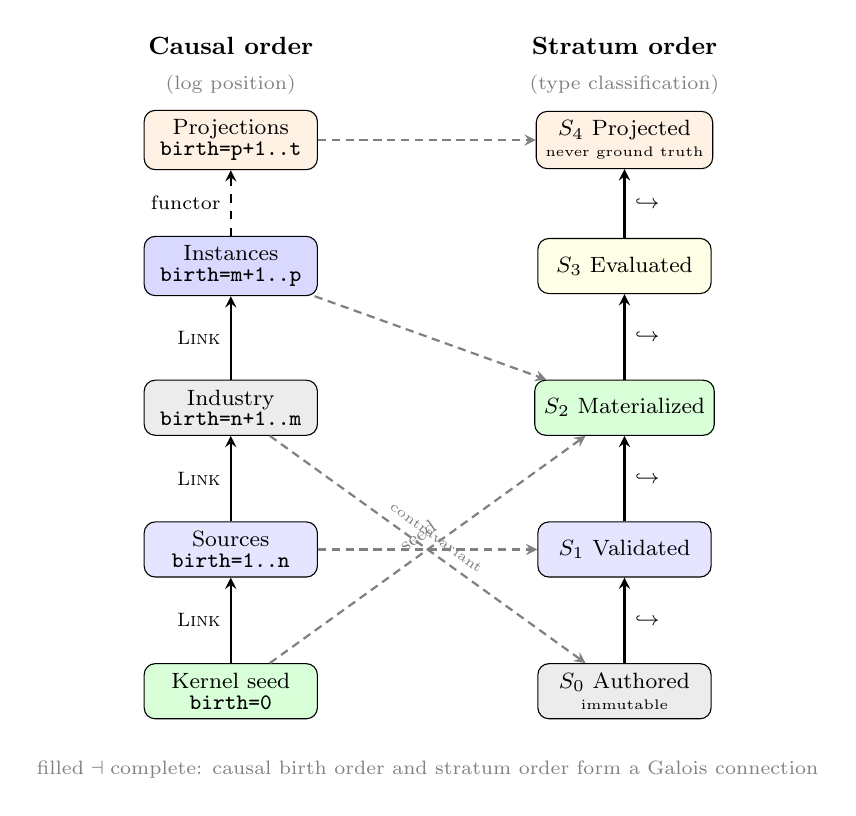
\begin{tikzpicture}[
  node/.style={draw, rounded corners, minimum width=2.2cm, minimum height=0.7cm, align=center, font=\footnotesize},
  arrow/.style={->, thick, >=stealth},
  cross/.style={->, thick, >=stealth, densely dashed, gray},
  lbl/.style={font=\scriptsize},
  col/.style={font=\small\bfseries}
]

% Column headers
\node[col] at (-2.5, 8.2) {Causal order};
\node[col] at (2.5, 8.2) {Stratum order};
\node[font=\scriptsize, text=gray] at (-2.5, 7.7) {(log position)};
\node[font=\scriptsize, text=gray] at (2.5, 7.7) {(type classification)};

% Left column: causal order (bottom = first, top = last)
\node[node, fill=green!15] (c0) at (-2.5, 0) {Kernel seed\\[-2pt] \texttt{birth=0}};
\node[node, fill=blue!10]  (c1) at (-2.5, 1.8) {Sources\\[-2pt] \texttt{birth=1..n}};
\node[node, fill=gray!15]  (c2) at (-2.5, 3.6) {Industry\\[-2pt] \texttt{birth=n+1..m}};
\node[node, fill=blue!15]  (c3) at (-2.5, 5.4) {Instances\\[-2pt] \texttt{birth=m+1..p}};
\node[node, fill=orange!10](c4) at (-2.5, 7.0) {Projections\\[-2pt] \texttt{birth=p+1..t}};

% Causal arrows (LINK authorization)
\draw[arrow] (c0) -- node[left, lbl] {\textsc{Link}} (c1);
\draw[arrow] (c1) -- node[left, lbl] {\textsc{Link}} (c2);
\draw[arrow] (c2) -- node[left, lbl] {\textsc{Link}} (c3);
\draw[arrow, dashed] (c3) -- node[left, lbl] {functor} (c4);

% Right column: stratum order (bottom = S0, top = S4)
\node[node, fill=gray!15]  (s0) at (2.5, 0) {$S_0$ Authored\\[-2pt] {\tiny immutable}};
\node[node, fill=blue!10]  (s1) at (2.5, 1.8) {$S_1$ Validated};
\node[node, fill=green!15] (s2) at (2.5, 3.6) {$S_2$ Materialized};
\node[node, fill=yellow!10](s3) at (2.5, 5.4) {$S_3$ Evaluated};
\node[node, fill=orange!10](s4) at (2.5, 7.0) {$S_4$ Projected\\[-2pt] {\tiny never ground truth}};

% Stratum inclusion arrows
\draw[arrow] (s0) -- node[right, lbl] {$\hookrightarrow$} (s1);
\draw[arrow] (s1) -- node[right, lbl] {$\hookrightarrow$} (s2);
\draw[arrow] (s2) -- node[right, lbl] {$\hookrightarrow$} (s3);
\draw[arrow] (s3) -- node[right, lbl] {$\hookrightarrow$} (s4);

% Cross-links showing contravariance (causal node → its stratum)
\draw[cross] (c0) -- node[above, lbl, sloped] {seed} (s2);
\draw[cross] (c1) -- (s1);
\draw[cross] (c2) -- node[above, lbl, sloped] {\tiny contravariant} (s0);
\draw[cross] (c3) -- (s2);
\draw[cross] (c4) -- (s4);

% Galois connection annotation (bottom)
\node[font=\scriptsize, text=gray, align=center] at (0, -1.0)
  {$\mathrm{filled} \dashv \mathrm{complete}$: causal birth order and
   stratum order form a Galois connection};

\end{tikzpicture}
\caption{Contravariant orders. \emph{Left}: the causal filtration ordered by
log position (Def.~\ref{def:causal-filtration}). \emph{Right}: the stratum
filtration ordered by type classification (Def.~\ref{def:stratum-filtration}).
Dashed cross-links map each causal stage to its stratum, revealing the
contravariance: the kernel seed is causally first but resides at~$S_2$, while
$S_0$ industry entities are causally posterior but immutable. The pair
$(\mathrm{filled}, \mathrm{complete})$ forms a Galois connection
(Prop.~\ref{prop:contravariant}) between these two independent orders.}
\label{fig:filtration}
\end{figure}


%% -----------------------------------------------------------------
\section{The Semantic Bottleneck and Invariant Morphisms}
\label{sec:bottleneck}

% Figure 3: Semantic Bottleneck — Task Decomposition vs Functorial Composition
\begin{figure}[t]
\centering
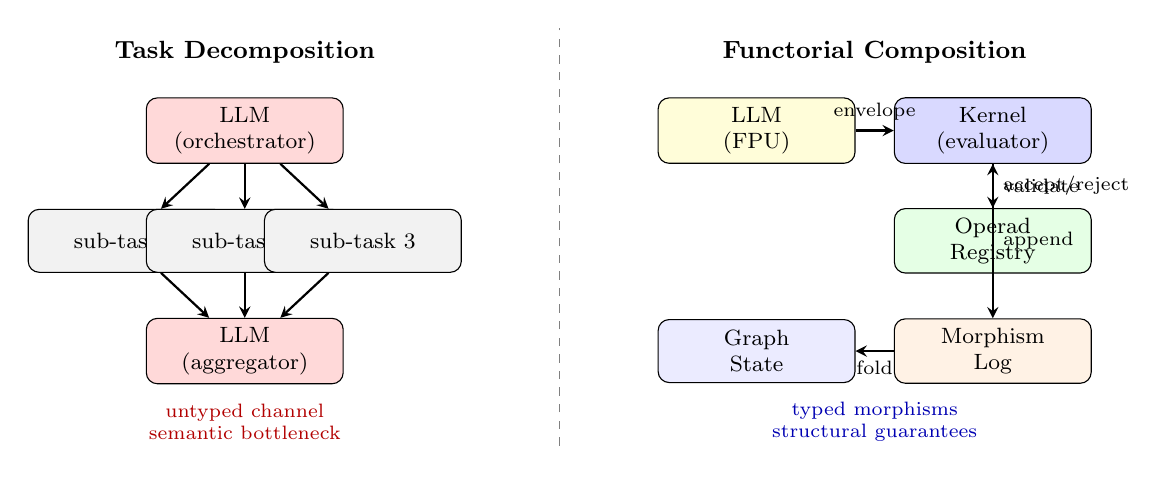
\begin{tikzpicture}[
  box/.style={draw, rounded corners, minimum width=2.5cm, minimum height=0.8cm, align=center, font=\footnotesize},
  arrow/.style={->, thick, >=stealth},
  label/.style={font=\scriptsize}
]

% Left side: Task Decomposition
\node[font=\small\bfseries] at (-4, 4.2) {Task Decomposition};

\node[box, fill=red!15] (llm1) at (-4, 3.2) {LLM\\(orchestrator)};
\node[box, fill=gray!10] (t1) at (-5.5, 1.8) {sub-task 1};
\node[box, fill=gray!10] (t2) at (-4, 1.8) {sub-task 2};
\node[box, fill=gray!10] (t3) at (-2.5, 1.8) {sub-task 3};
\node[box, fill=red!15] (agg) at (-4, 0.4) {LLM\\(aggregator)};

\draw[arrow] (llm1) -- (t1);
\draw[arrow] (llm1) -- (t2);
\draw[arrow] (llm1) -- (t3);
\draw[arrow] (t1) -- (agg);
\draw[arrow] (t2) -- (agg);
\draw[arrow] (t3) -- (agg);

\node[label, text=red!70!black, align=center] at (-4, -0.5) {untyped channel\\semantic bottleneck};

% Divider
\draw[dashed, gray] (0, -0.8) -- (0, 4.5);

% Right side: Functorial Composition
\node[font=\small\bfseries] at (4, 4.2) {Functorial Composition};

\node[box, fill=yellow!15] (fpu) at (2.5, 3.2) {LLM\\(FPU)};
\node[box, fill=blue!15] (kernel) at (5.5, 3.2) {Kernel\\(evaluator)};
\node[box, fill=green!10] (reg) at (5.5, 1.8) {Operad\\Registry};
\node[box, fill=orange!10] (log) at (5.5, 0.4) {Morphism\\Log};
\node[box, fill=blue!8] (state) at (2.5, 0.4) {Graph\\State};

\draw[arrow] (fpu) -- node[above, label] {envelope} (kernel);
\draw[arrow] (kernel) -- node[right, label] {validate} (reg);
\draw[arrow, dashed] (reg) -- node[right, label] {accept/reject} (kernel);
\draw[arrow] (kernel) -- node[right, label] {append} (log);
\draw[arrow] (log) -- node[below, label] {fold} (state);

\node[label, text=blue!70!black, align=center] at (4, -0.5) {typed morphisms\\structural guarantees};

\end{tikzpicture}
\caption{The semantic bottleneck (left): LLMs serve as both orchestrator and
aggregator through an untyped channel, producing brittle compositions.
Functorial composition (right): the LLM acts as a Fuzzy Processing Unit
emitting typed morphism envelopes, validated by the operad registry before
commitment to the append-only log.}
\label{fig:bottleneck}
\end{figure}


\subsection{The Semantic Bottleneck}

The prevailing paradigm for multi-agent orchestration relies on the LLM's
embedding space as both computation engine and state router. We formalize this
structural failure as the \emph{semantic bottleneck}: a system architecture
where semantic inference and operational state management share a single,
untyped channel. As task complexity grows, this channel saturates, producing
hallucinated execution paths and brittle error recovery.

\subsection{Four Invariant Natural Transformations}

\texttt{mo:os} resolves the bottleneck by restricting all state mutations to
exactly four natural transformations:

\begin{center}
\begin{tabular}{@{}llll@{}}
\toprule
NT & Signature & Semantic & Guard \\
\midrule
\textsc{Add}    & $\varnothing \to \mathrm{Node}$ & Create node &
  Duplicate URN $\Rightarrow$ \texttt{ErrNodeExists} \\
\textsc{Link}   & $N \times N \to \mathrm{Wire}$ & Create wire &
  Operadic port validation \\
\textsc{Mutate} & $N \to N$ & Update payload &
  Version CAS + $S_0$ block \\
\textsc{Unlink} & $\mathrm{Wire} \to \varnothing$ & Remove wire &
  Wire not found $\Rightarrow$ error \\
\bottomrule
\end{tabular}
\end{center}

These four operations are \emph{complete}: any graph state reachable from the
empty graph can be expressed as a finite composition of \textsc{Add},
\textsc{Link}, \textsc{Mutate}, and \textsc{Unlink} envelopes. The LLM (as
FPU) proposes candidate envelopes; the kernel validates and commits them.

\subsection{Operadic Validation}

The semantic registry $\mathcal{R}$ is an operad algebra over the port
structure of $\mathcal{C}$. For each type $\tau \in \mathcal{T}$, the registry
specifies:
\begin{itemize}
  \item \textbf{Allowed strata}: the set of valid strata for instances of $\tau$.
  \item \textbf{Port specifications}: for each named port, its direction
        (in/out) and admissible target types.
  \item \textbf{Mutability}: whether instances admit \textsc{Mutate}.
\end{itemize}

A \textsc{Link} envelope $w\colon n_1 \xrightarrow{(p_s, p_t)} n_2$ is valid
if and only if: (1) $p_s$ exists on $\tau(n_1)$ with direction ``out'', (2)
$p_t$ exists on $\tau(n_2)$ with direction ``in'', and (3) $(\tau(n_2), p_t)$
is in the admissible target set of $p_s$. This three-part check implements the
operadic composition constraints of $\mathcal{W}$.

%% -----------------------------------------------------------------
\section{The Recursive Semantic Bridge}
\label{sec:bridge}

We formalize the \texttt{mo:os} architecture as a realization of Lawvere's
functorial semantics. The database graph serves as the abstract syntax tree
(AST) of our language.

\begin{definition}[Syntax Category]
$\mathbf{Syn}$ has objects = Container types (the 21 kinds of the ontology)
and morphisms = wiring diagrams (the 16 morphism types).
\end{definition}

\begin{definition}[Semantics Category]
$\mathbf{Sem}$ has objects = Go runtime states and morphisms = deterministic
kernel evaluations (the fold step of Equation~\ref{eq:cata}).
\end{definition}

The \emph{Recursive Semantic Bridge} is the structure-preserving functor:
\begin{equation}
F\colon \mathbf{Syn} \to \mathbf{Sem}
\end{equation}

\begin{equation}
\begin{tikzcd}
\mathbf{Syn} \arrow[r, "F"] \arrow[d, "\alpha"'] & \mathbf{Sem} \arrow[d, "F(\alpha)"] \\
\mathbf{Syn}' \arrow[r, "F"'] & \mathbf{Sem}'
\end{tikzcd}
\end{equation}

where $\alpha$ represents a morphism (state transition) in the syntax, and
$F(\alpha)$ is the corresponding Go kernel evaluation. The functor preserves
composition: applying two morphisms sequentially in $\mathbf{Syn}$ yields the
same result as applying their $F$-images sequentially in $\mathbf{Sem}$.

% Figure 2: Hydration Pipeline — Stratum Promotion
% S0 (Authored) → S1 (Validated) → S2 (Materialized) → S3 (Evaluated) → S4 (Projected)
\begin{figure}[t]
\centering
\begin{tikzcd}[column sep=2.2cm, row sep=0.8cm]
  S_0 \arrow[r, "\text{schema}"] \arrow[d, phantom, "{\text{\footnotesize JSON files}}"']
  & S_1 \arrow[r, "\text{Materialize}"] \arrow[d, phantom, "{\text{\footnotesize validated}}"']
  & S_2 \arrow[r, "\text{ApplyProgram}"] \arrow[d, phantom, "{\text{\footnotesize programs}}"']
  & S_3 \arrow[r, "\text{Scope}"] \arrow[d, phantom, "{\text{\footnotesize graph state}}"']
  & S_4 \arrow[d, phantom, "{\text{\footnotesize projections}}"']
  \\
  \text{\footnotesize Authored}
  & \text{\footnotesize Validated}
  & \text{\footnotesize Materialized}
  & \text{\footnotesize Evaluated}
  & \text{\footnotesize Projected}
\end{tikzcd}
\caption{The hydration pipeline as stratum promotion. Each stage corresponds to
a kernel operation: schema validation ($S_0 \to S_1$), materialization into
Programs ($S_1 \to S_2$), fold evaluation ($S_2 \to S_3$), and scoped
projection via BFS ($S_3 \to S_4$). $S_4$ outputs are never ground truth.}
\label{fig:hydration}
\end{figure}


\subsection{Hydration as Stratum Promotion}

The hydration pipeline maps directly onto the stratum lattice:

\begin{center}
\begin{tabular}{@{}lll@{}}
\toprule
Stage & Stratum & Kernel Operation \\
\midrule
Authored   & $S_0$ & JSON instance files on disk \\
Validated  & $S_1$ & Schema check (JSON Schema draft-07) \\
Materialized & $S_2$ & \texttt{Materialize}: instance $\to$ Program \\
Evaluated  & $S_3$ & \texttt{ApplyProgram}: fold into graph state \\
Projected  & $S_4$ & \texttt{ScopedSubgraph}: BFS lens \\
\bottomrule
\end{tabular}
\end{center}

The key invariant is that $S_4$ projections are \emph{never} ground truth:
they are views derived from the evaluated state, and the graph can always be
reconstructed from the morphism log via replay (Equation~\ref{eq:cata}).

\subsection{Harness Agnosticism}

Because the functor $F$ maps syntax to semantics uniformly, any external
tool---an LLM, a database, a UI framework---is merely an object in
$\mathbf{Syn}$ whose interaction with the graph is governed by $F$. This
achieves \emph{harness agnosticism}: the UI surface is a direct, consistent
projection of the categorical state, requiring no intermediary state-management
synchronization. Nested sub-workspaces are submodules in the categorical
composition, inheriting structural integrity via algebraic closure.

% Figure 4: Three-Layer Tower — Translation Functors from Industry to Kernel
% Industry (SynBN) → Superset (SynLP) → Kernel (promoted projections)
\begin{figure}[t]
\centering
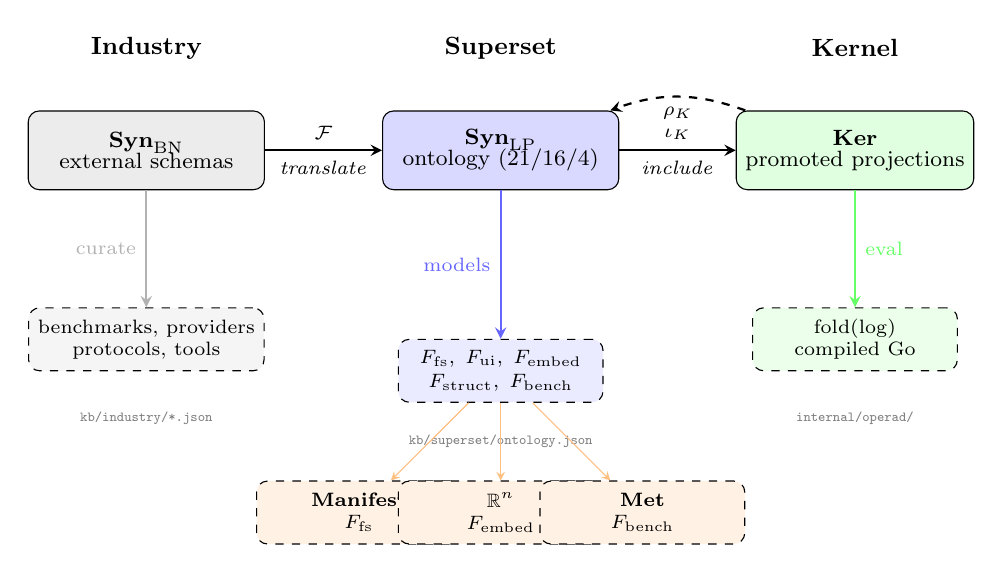
\begin{tikzpicture}[
  box/.style={draw, rounded corners, minimum width=3.0cm, minimum height=1.0cm, align=center, font=\footnotesize},
  sem/.style={draw, rounded corners, dashed, minimum width=2.6cm, minimum height=0.8cm, align=center, font=\scriptsize},
  arrow/.style={->, thick, >=stealth},
  functor/.style={->, thick, >=stealth, font=\small},
  label/.style={font=\scriptsize},
  col/.style={font=\small\bfseries}
]

% Column headers
\node[col] at (-4.5, 4.5) {Industry};
\node[col] at (0, 4.5) {Superset};
\node[col] at (4.5, 4.5) {Kernel};

% Top row: Syntax categories
\node[box, fill=gray!15] (ind) at (-4.5, 3.2) {$\mathbf{Syn}_{\mathrm{BN}}$\\[-2pt] external schemas};
\node[box, fill=blue!15] (sup) at (0, 3.2) {$\mathbf{Syn}_{\mathrm{LP}}$\\[-2pt] ontology (21/16/4)};
\node[box, fill=green!12] (ker) at (4.5, 3.2) {$\mathbf{Ker}$\\[-2pt] promoted projections};

% Horizontal functor arrows (translation)
\draw[functor] (ind) -- node[above, label] {$\mathcal{F}$} node[below, label] {\textit{translate}} (sup);
\draw[functor] (sup) -- node[above, label] {$\iota_K$} node[below, label] {\textit{include}} (ker);

% Adjoint arrow (restrict) — dashed, below
\draw[functor, dashed, bend right=20] (ker) to node[below, label] {$\rho_K$} node[above, label] {} (sup);

% Bottom row: Semantic models (functor images)
\node[sem, fill=gray!8] (sem-ind) at (-4.5, 0.8) {benchmarks, providers\\protocols, tools};
\node[sem, fill=blue!8] (sem-sup) at (0, 0.4) {$F_{\mathrm{fs}},\; F_{\mathrm{ui}},\; F_{\mathrm{embed}}$\\[1pt] $F_{\mathrm{struct}},\; F_{\mathrm{bench}}$};
\node[sem, fill=green!8] (sem-ker) at (4.5, 0.8) {$\mathrm{fold}(\mathrm{log})$\\compiled Go};

% Vertical functor arrows (syntax → semantics)
\draw[arrow, gray!60] (ind) -- node[left, label] {curate} (sem-ind);
\draw[arrow, blue!60] (sup) -- node[left, label] {models} (sem-sup);
\draw[arrow, green!60] (ker) -- node[right, label] {eval} (sem-ker);

% File path annotations (grounding in codebase)
\node[font=\tiny\ttfamily, text=gray] at (-4.5, -0.2) {kb/industry/*.json};
\node[font=\tiny\ttfamily, text=gray] at (0, -0.5) {kb/superset/ontology.json};
\node[font=\tiny\ttfamily, text=gray] at (4.5, -0.2) {internal/operad/};

% Target categories fan-out from superset
\node[sem, fill=orange!10] (t1) at (-1.8, -1.4) {\textbf{Manifest}\\$F_{\mathrm{fs}}$};
\node[sem, fill=orange!10] (t2) at (0, -1.4) {$\mathbb{R}^n$\\$F_{\mathrm{embed}}$};
\node[sem, fill=orange!10] (t3) at (1.8, -1.4) {\textbf{Met}\\$F_{\mathrm{bench}}$};

\draw[arrow, orange!50, thin] (sem-sup) -- (t1);
\draw[arrow, orange!50, thin] (sem-sup) -- (t2);
\draw[arrow, orange!50, thin] (sem-sup) -- (t3);

\end{tikzpicture}
\caption{The three-layer tower. Industry data enters via the translation functor
$\mathcal{F}\colon \mathbf{Syn}_{\mathrm{BN}} \to \mathbf{Syn}_{\mathrm{LP}}$.
The superset ontology serves as the free category whose models (FUN01--FUN05) are
structure-preserving functors to target categories. Stable patterns are promoted
into the kernel via $\iota_K$; the kernel exposes its structure back to the graph
via $\rho_K$ (the adjoint restriction). File paths ground each layer in the
codebase.}
\label{fig:tower}
\end{figure}


\subsection{LLM as Endofunctor}
\label{subsec:llm-endofunctor}

In \texttt{mo:os}, an LLM is not an orchestrator but an object of type
\texttt{agnostic\_model} in $\mathcal{C}$. Its interface to the rest of the
graph is mediated entirely by \textsc{CAN\_ROUTE} morphisms connecting it to
\texttt{protocol\_adapter} nodes. This embedding has a precise categorical
reading: the LLM acts as an endofunctor on the subcategory of morphism
proposals, accepting candidate envelopes and returning refined candidates---all
subject to the kernel's validation.

The \emph{benchmark functor} $F_{\mathrm{bench}}$ formalizes model selection as
a functorial problem. Let $\mathcal{C}_{\mathrm{Prov}}$ be the full
subcategory of $\mathcal{C}$ whose objects are of type \texttt{provider} and
whose morphisms are feature-bearing wires (e.g., \textsc{CAN\_ROUTE},
\textsc{BENCHMARKS\_ON}).

\begin{definition}[Benchmark Functor]
\label{def:benchmark-functor}
The benchmark functor $F_{\mathrm{bench}}\colon \mathcal{C}_{\mathrm{Prov}} \to
\mathbf{Met}$ maps:
\begin{itemize}
  \item Each provider object $p$ to a point in the metric space
        $(\mathbb{R}^k, d)$ representing its benchmark score vector (latency,
        accuracy, cost, throughput).
  \item Each feature morphism $f\colon p_1 \to p_2$ to a non-expansive map
        preserving the partial order on scores.
\end{itemize}
\end{definition}

Model selection then reduces to choosing the provider whose
$F_{\mathrm{bench}}$-image optimizes a given objective. This is the
\emph{collider pattern}: models are benchmarked agnostically as objects in the
graph, their capabilities are morphisms, and composition of model pipelines
happens categorically through the typed wiring algebra---not through prompt
engineering or ad-hoc orchestration scripts.

%% -----------------------------------------------------------------
\section{System~3: Multi-Path DAG Reasoning}
\label{sec:system3}

We extend LogicGraph \cite{logicgraph2025} to define System~3 reasoning over
the morphism space:

\begin{itemize}
  \item \textbf{System~1}: Intuitive token prediction (standard LLM inference).
  \item \textbf{System~2}: Linear chain-of-thought (sequential reasoning).
  \item \textbf{System~3}: DAG exploration over typed morphism space.
\end{itemize}

In System~3, the deterministic kernel spawns candidate sub-graphs where each
edge is a structure-preserving morphism validated against the operad registry.
By applying tree search heuristics (MCTS or beam search) over the morphism
space, \texttt{mo:os} simulates branching future states. Because each branch
is restricted to valid categorical syntax, the search space is automatically
pruned of structurally inconsistent outcomes.

This enables high-stakes reasoning---infrastructure deployment, data
migration, multi-step planning---where the error surface of a single LLM
prompt would be prohibitively large. The typed morphism space provides a
natural pruning function: invalid compositions are rejected before evaluation,
and the catamorphic replay guarantees that any accepted path can be audited.

%% -----------------------------------------------------------------
\section{Implementation}
\label{sec:implementation}

% Figure 1: mo:os Kernel Architecture — Layered Separation
% Pure core (no IO) → Effect shell (RWMutex) → HTTP transport
\begin{figure}[t]
\centering
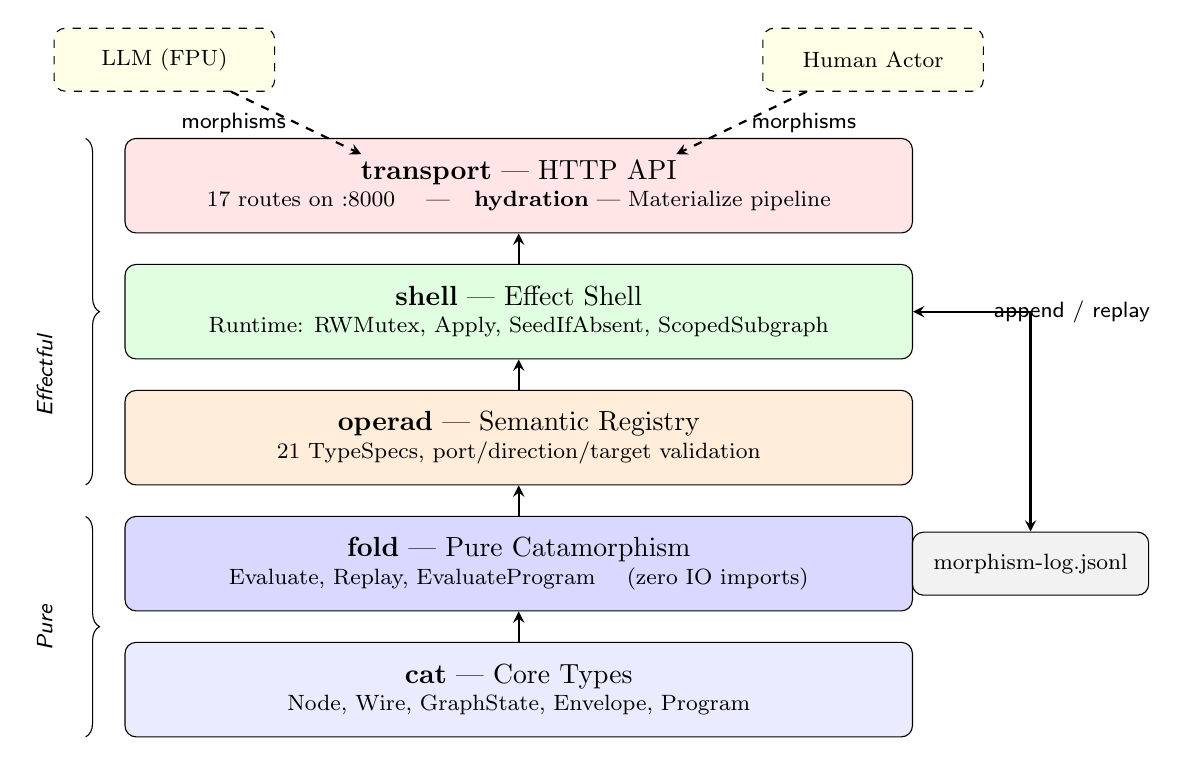
\begin{tikzpicture}[
  layer/.style={draw, rounded corners, minimum width=10cm, minimum height=1.2cm, align=center},
  arrow/.style={->, thick, >=stealth},
  label/.style={font=\footnotesize\sffamily}
]

% Layers (bottom to top)
\node[layer, fill=blue!8] (types) at (0,0) {\textbf{cat} — Core Types\\[-2pt]
  \footnotesize Node, Wire, GraphState, Envelope, Program};

\node[layer, fill=blue!15] (fold) at (0,1.6) {\textbf{fold} — Pure Catamorphism\\[-2pt]
  \footnotesize Evaluate, Replay, EvaluateProgram \quad (zero IO imports)};

\node[layer, fill=orange!15] (operad) at (0,3.2) {\textbf{operad} — Semantic Registry\\[-2pt]
  \footnotesize 21 TypeSpecs, port/direction/target validation};

\node[layer, fill=green!12] (shell) at (0,4.8) {\textbf{shell} — Effect Shell\\[-2pt]
  \footnotesize Runtime: RWMutex, Apply, SeedIfAbsent, ScopedSubgraph};

\node[layer, fill=red!10] (transport) at (0,6.4) {\textbf{transport} — HTTP API\\[-2pt]
  \footnotesize 17 routes on :8000 \quad|\quad \textbf{hydration} — Materialize pipeline};

% Arrows
\draw[arrow] (types) -- (fold);
\draw[arrow] (fold) -- (operad);
\draw[arrow] (operad) -- (shell);
\draw[arrow] (shell) -- (transport);

% Side labels
\node[label, rotate=90, anchor=south] at (-5.8,0.8) {\textit{Pure}};
\node[label, rotate=90, anchor=south] at (-5.8,4.0) {\textit{Effectful}};

% Brace for pure section
\draw[decorate, decoration={brace, amplitude=5pt, mirror}] (-5.5,-0.6) -- (-5.5,2.2);
\draw[decorate, decoration={brace, amplitude=5pt, mirror}] (-5.5,2.6) -- (-5.5,7.0);

% External actors
\node[draw, dashed, rounded corners, minimum width=2.8cm, minimum height=0.8cm, fill=yellow!10] (llm) at (-4.5,8.0) {\footnotesize LLM (FPU)};
\node[draw, dashed, rounded corners, minimum width=2.8cm, minimum height=0.8cm, fill=yellow!10] (human) at (4.5,8.0) {\footnotesize Human Actor};

\draw[arrow, dashed] (llm) -- node[left, label] {morphisms} (-2,6.8);
\draw[arrow, dashed] (human) -- node[right, label] {morphisms} (2,6.8);

% JSONL log
\node[draw, rounded corners, minimum width=3cm, minimum height=0.8cm, fill=gray!10] (log) at (6.5,1.6) {\footnotesize morphism-log.jsonl};
\draw[arrow, <->] (shell.east) -| node[right, label, pos=0.3] {append / replay} (log);

\end{tikzpicture}
\caption{Layered architecture of the \texttt{mo:os} kernel. The pure core
(\texttt{cat} + \texttt{fold}) contains zero IO imports. The effect shell
wraps it with \texttt{sync.RWMutex} for concurrent access. Both LLM agents
and human actors interact exclusively through typed morphism envelopes.}
\label{fig:architecture}
\end{figure}


\texttt{mo:os} is implemented in Go (1.22+) as a single-binary kernel with
zero external dependencies beyond the standard library. The architecture
separates pure computation from effectful state management:

\begin{center}
\begin{tabular}{@{}llp{5cm}@{}}
\toprule
Layer & Package & Responsibility \\
\midrule
Types      & \texttt{cat}       & Core types: Node, Wire, GraphState, Envelope, Program. 4 morphism types, 5 strata. \\
Pure fold  & \texttt{fold}      & Catamorphism: \texttt{Evaluate}, \texttt{Replay}. Zero IO imports. \\
Operad     & \texttt{operad}    & Semantic registry: 21 TypeSpecs with port/direction/target validation. \\
Effect shell & \texttt{shell}   & \texttt{Runtime}: RWMutex-guarded state, \texttt{Apply}, \texttt{SeedIfAbsent}. \\
Transport  & \texttt{transport} & 17 HTTP routes on port 8000. Embedded Explorer UI via \texttt{go:embed} (\texttt{transport/static/}). \\
Hydration  & \texttt{hydration} & \texttt{Materialize}: instance JSON $\to$ Program. \texttt{HydrateAll}: batch boot. \\
Lens       & \texttt{lens}      & Composable graph filter: \texttt{Apply(spec, state)}, 5 predicate types (kind, stratum, category, port, neighborhood), scope composition. \\
MCP bridge & \texttt{mcp}       & MCP server on port 8080: SSE transport, JSON-RPC 2.0, 5 tool schemas. \\
Functor    & \texttt{functor}   & Benchmark functor FUN05: $\mathcal{C}_{\mathrm{Prov}} \to \mathbf{Met}$. \\
\bottomrule
\end{tabular}
\end{center}

\subsection{Catamorphic Replay}

The morphism log is an append-only JSONL file. State reconstruction is a left
fold:

\begin{lstlisting}[language=Go,caption={Pure replay (simplified)}]
func Replay(log []Envelope) GraphState {
    state := NewGraphState() // empty
    for _, env := range log {
        state = Evaluate(state, env)
    }
    return state
}
\end{lstlisting}

The \texttt{fold} package imports no IO packages (\texttt{os}, \texttt{net},
\texttt{sync}); it operates purely on values. The effect shell
(\texttt{shell.Runtime}) wraps the pure fold with \texttt{sync.RWMutex} for
concurrent read access and exclusive write access.

\subsection{Idempotent Seeding}

Boot uses \texttt{SeedIfAbsent}, which absorbs \texttt{ErrNodeExists} and
\texttt{ErrWireExists}. This makes repeated boots idempotent: the first boot
creates 13 seed morphisms; subsequent boots replay the log and produce zero
new entries.

\subsection{MCP Bridge as Natural Transformation}
\label{subsec:mcp-bridge}

The Model Context Protocol (MCP) bridge \cite{mcp2024} exposes the kernel to
LLM tool-use via SSE on port 8080. We formalize this bridge as a natural
transformation between two categories.

\begin{definition}[Kernel and Tool Categories]
Let $\mathcal{C}_K$ be the category whose objects are graph operations
(\textup{\textsc{Add}}, \textup{\textsc{Link}}, \textup{\textsc{Mutate}}, \textup{\textsc{Unlink}}, and the
read operations \textup{\textsc{State}}, \textup{\textsc{Lookup}}, \textup{\textsc{Scope}}) and whose
morphisms are kernel evaluations (applications of the catamorphic fold). Let
$\mathcal{C}_L$ be the category whose objects are JSON tool schemas and whose
morphisms are JSON-RPC 2.0 invocations.
\end{definition}

\begin{definition}[MCP Natural Transformation]
The MCP bridge is a natural transformation $\eta\colon \mathcal{C}_K
\Rightarrow \mathcal{C}_L$ whose five components are:
\begin{center}
\begin{tabular}{@{}ll@{}}
\toprule
Component $\eta_i$ & Kernel operation $\to$ Tool schema \\
\midrule
$\eta_{\mathrm{state}}$     & \textup{\textsc{State}} $\mapsto$ \texttt{graph\_state} \\
$\eta_{\mathrm{lookup}}$    & \textup{\textsc{Lookup}} $\mapsto$ \texttt{node\_lookup} \\
$\eta_{\mathrm{apply}}$     & \textup{\textsc{Apply}} $\mapsto$ \texttt{apply\_morphism} \\
$\eta_{\mathrm{scope}}$     & \textup{\textsc{Scope}} $\mapsto$ \texttt{scoped\_subgraph} \\
$\eta_{\mathrm{bench}}$     & \textup{\textsc{Benchmark}} $\mapsto$ \texttt{benchmark\_project} \\
\bottomrule
\end{tabular}
\end{center}
\end{definition}

The naturality condition states that for any kernel morphism $f\colon A \to B$
in $\mathcal{C}_K$:
\begin{equation}
\label{eq:naturality-mcp}
\begin{tikzcd}
\mathcal{C}_K(A) \arrow[r, "\eta_A"] \arrow[d, "f"'] & \mathcal{C}_L(\eta_A) \arrow[d, "\eta(f)"] \\
\mathcal{C}_K(B) \arrow[r, "\eta_B"'] & \mathcal{C}_L(\eta_B)
\end{tikzcd}
\end{equation}

Concretely: applying a morphism in the kernel and then projecting the result
via an MCP tool yields the same output as first projecting via the tool and
then applying the corresponding JSON-RPC invocation. This ensures that LLM
clients observe a consistent view of the kernel state regardless of whether
they query before or after a mutation is committed.

\subsection{Pipeline Complexity and Subgraph Metrics}
\label{subsec:pipeline-complexity}

The scoped subgraph operation (Section~\ref{sec:container}) enables us to
define formal complexity metrics for pipeline reasoning.

\begin{definition}[Subgraph Cost Model]
For an actor $a$ with scoped subgraph $G_a = \mathrm{ScopedSubgraph}(a)$,
define:
\begin{itemize}
  \item \emph{Discovery cost}: $D(G_a) \propto |E(G_a)|$ --- the cost of
        scanning edges to discover structural relationships.
  \item \emph{Retrieval cost}: $R(G_a) \propto |V(G_a)|$ --- the cost of
        accessing node state within the scope.
  \item \emph{Complexity ratio}: $\kappa(G_a) = |E(G_a)| / |V(G_a)|$ ---
        the average edge density per node, measuring wiring complexity.
\end{itemize}
\end{definition}

The BFS scoping algorithm computes $G_a$ in $O(|V| + |E|)$ time under
\texttt{RLock}, where $|V|$ and $|E|$ are the sizes of the full graph. Once
scoped, all subsequent operations on $G_a$ operate on the reduced subgraph.

\begin{theorem}[Discovery Cost Reduction]
\label{thm:discovery-cost}
Let $E_{\mathrm{total}}$ be the edge set of the full graph and
$E_{\mathrm{scope}} = E(G_a) \subseteq E_{\mathrm{total}}$ be the edge set
of the scoped subgraph induced by the ownership functor. The transition from
task decomposition (which must inspect all edges to discover relevant
structure) to functorial composition via scoped projection reduces discovery
cost from $O(|E_{\mathrm{total}}|)$ to $O(|E_{\mathrm{scope}}|)$.
\end{theorem}

\begin{proof}[Proof sketch]
Task decomposition frameworks lack an ownership functor and must traverse the
full graph to determine which edges are relevant to a given actor. The
ownership functor $\Omega\colon \mathcal{C} \to \mathbf{Forest}$ partitions
the graph into disjoint subtrees. For any actor $a$, the scoped subgraph
$G_a = \Omega^{-1}(a)$ contains exactly those edges internal to $a$'s
ownership subtree. Since $\Omega$ is computed once during BFS and the result
is cached, subsequent discovery within $G_a$ examines only
$|E_{\mathrm{scope}}|$ edges. The ratio
$|E_{\mathrm{scope}}|/|E_{\mathrm{total}}|$ is bounded by the ownership
fraction of the actor, which in practice is $\ll 1$ for large graphs.
\end{proof}

\subsection{Data Lens: Functorial Projection as a User Interface}
\label{subsec:data-lens}

The \texttt{lens} package materializes functorial projection as a composable
query interface. A \emph{lens specification} $L = (\rho_1, \ldots, \rho_n, m)$
pairs a sequence of predicates over kind, stratum, category, port, or
$k$-hop neighbourhood with a composition mode $m \in \{\cap, \cup\}$.
For scoped queries the kernel first applies the ownership functor
$\Omega$ (Section~\ref{sec:container}), then applies $\Lambda$ (lens filter):
the composed functor $\Lambda \circ \Omega \colon \mathcal{C} \to
\mathcal{C}_{\mathrm{filtered}}$ is served via \texttt{GET /state/lens} and
\texttt{POST /state/lens}.

The Explorer UI renders the filtered \texttt{GraphState} as structured tables
grouped by object kind, morphism type, type registry, and morphism history.
This design makes categorical structure legible through tabular projection
rather than spatial layout, demonstrating that functorial composition provides
auditable structure \emph{without} requiring a dedicated hypergraph renderer.

\subsection{Metrics}

\begin{center}
\begin{tabular}{@{}lr@{}}
\toprule
Metric & Value \\
\midrule
Go source lines & ${\sim}4{,}000$ \\
Ontology object kinds & 21 \\
Ontology morphism types & 16 \\
Invariant natural transformations & 4 \\
Strata & 5 \\
Categories & 22 \\
Functors & 5 \\
HTTP routes & 17 \\
MCP tools & 5 \\
Nodes (post-hydration) & 118 \\
Wires (post-hydration) & 131 \\
Test packages (all green) & 9 \\
External dependencies & 0 \\
\bottomrule
\end{tabular}
\end{center}

%% -----------------------------------------------------------------
\section{Related Work}
\label{sec:related}

\paragraph{Categorical frameworks.}
Catlab \cite{catlab2024} provides Julia libraries for computational category
theory; Statebox \cite{statebox2019} applies Petri nets to blockchain
consensus; Lynch and Breiner \cite{lynch2023nested} implement nested wiring
diagrams in Semagrams. None target the operational gap between LLM inference
and runtime graph state management.

\paragraph{Multi-agent orchestration.}
LangChain, CrewAI, AutoGen, and LangGraph rely on LLM-driven task
decomposition. These frameworks lack formal structural guarantees: correctness
depends on the LLM maintaining coherent state across unbounded context windows.

\paragraph{Operadic composition.}
Spivak's wiring diagram operads \cite{spivak2013,spivak2013operad} and Yau's
finite presentation results \cite{yau2018} provide the mathematical foundation
for our port-typed composition. Shapiro et al.'s dynamic operads
\cite{shapiro2022} formalize how operadic structure evolves---a pattern
\texttt{mo:os} realizes through its mutable graph topology.

\paragraph{Functorial semantics for computation.}
Bonchi et al.\ \cite{bonchi2017functorial} extend functorial semantics to
relational theories. Gu and Zanasi \cite{gu2021functorial} apply functorial
semantics as a unifying framework for logic programming. \texttt{mo:os}
applies these ideas to AI-human computation, where the ``programs'' are
morphism envelopes emitted by both human actors and LLM agents.

\paragraph{Category theory for AI.}
Pan \cite{pan2024token} proposes a categorical framework at the token level of
transformer architectures. Gavranovi{\'c} et al.\ \cite{gavranovic2024categorical}
develop an algebraic theory of deep learning architectures using 2-categories
of parametric maps. These works formalize AI \emph{internals} categorically;
\texttt{mo:os} instead formalizes the \emph{interface} between AI agents and
shared state.

\paragraph{Neuro-symbolic reasoning.}
LogicGraph \cite{logicgraph2025} benchmarks multi-path reasoning in
high-dimensional search spaces. \texttt{mo:os}'s System~3 extends this by
embedding DAG reasoning within a categorically typed morphism space, providing
structural pruning guarantees absent in untyped search.

%% -----------------------------------------------------------------
\section{Conclusion}
\label{sec:conclusion}

We have demonstrated that the transition from top-down task decomposition to
bottom-up functorial composition provides a rigorous foundation for
AI-human computation. By anchoring LLMs as coprocessors within a typed
categorical kernel, \texttt{mo:os} resolves the semantic bottleneck while
preserving the expressiveness needed for complex multi-agent workflows.

The working implementation---approximately 4{,}000 lines of Go with zero
dependencies, 21 object kinds validated by an operad registry, 118 nodes and
131 wires post-hydration, and deterministic catamorphic replay---shows that
mathematical rigor is not an obstacle to practical systems but rather their
most robust enabling technology.
The authority filtration (Theorem~\ref{thm:authority}) and contravariant
orders (Proposition~\ref{prop:contravariant}) upgrade the governance axiom
from a design principle to a pair of formal results: every node's provenance
is auditable by tracing \textsc{Link} morphisms back through the causal
filtration to the kernel seed, and the Galois connection between causal birth
order and stratum classification provides a formal tool for boot sequencing
and structural consistency verification.
The MCP bridge (Section~\ref{subsec:mcp-bridge}) realizes the natural
transformation $\eta\colon \mathcal{C}_K \Rightarrow \mathcal{C}_L$, making
the kernel's categorical operations directly accessible to any MCP-compliant
LLM client via five tool schemas over SSE and JSON-RPC 2.0. The benchmark
functor $F_{\mathrm{bench}}\colon \mathcal{C}_{\mathrm{Prov}} \to
\mathbf{Met}$ (Definition~\ref{def:benchmark-functor}) reduces model selection
to a functorial optimization problem, and the pipeline complexity metrics
(Theorem~\ref{thm:discovery-cost}) formalize the cost advantage of scoped
projection over full-graph traversal.

Future work includes:
(1)~upgrading the transport layer to HTTP/3 via \texttt{quic-go}
\cite{rfc9114}, mapping stratum-specific reliability requirements to
independent QUIC streams;
(2)~pipeline complexity metrics based on the subgraph $|E|/|V|$ ratio,
enabling automatic detection of over-wired subsystems;
(3)~LLM-as-morphism formalization, embedding \texttt{agnostic\_model} inference
as a first-class endomorphism in the typed graph;
and (4)~quantitative comparison of morphism-based error recovery rates against
traditional LLM orchestration frameworks such as LangChain and AutoGen.

\bibliographystyle{eptcs}
\bibliography{references}

\end{document}
